\documentclass{article}

\usepackage[letterpaper, margin=0.5in]{geometry}


\usepackage{graphicx}
%\usepackage{lscape}

\begin{document}


\begin{figure}
  \includegraphics[width=0.33\textwidth]{Results/Lasso/lasso_lambda_set_trial1_dataset1.pdf}
  \includegraphics[width=0.33\textwidth]{Results/Lasso/lasso_lambda_set_trial1_dataset2.pdf}
  \includegraphics[width=0.33\textwidth]{Results/Lasso/lasso_lambda_set_trial1_dataset4.pdf} \\
  \includegraphics[width=0.33\textwidth]{Results/Lasso/lasso_lambda_set_trial2_dataset1.pdf}
  \includegraphics[width=0.33\textwidth]{Results/Lasso/lasso_lambda_set_trial2_dataset2.pdf}
  \includegraphics[width=0.33\textwidth]{Results/Lasso/lasso_lambda_set_trial2_dataset4.pdf} \\
  \includegraphics[width=0.33\textwidth]{Results/Lasso/lasso_lambda_set_trial3_dataset1.pdf}
  \includegraphics[width=0.33\textwidth]{Results/Lasso/lasso_lambda_set_trial3_dataset2.pdf}
  \includegraphics[width=0.33\textwidth]{Results/Lasso/lasso_lambda_set_trial3_dataset4.pdf}   
\caption{\label{fig:lassopath}Lasso regularization path for regression coefficients of the input features. Coefficient values deviating from zero suggest that the corresponding feature might be a significant indicator for MI risk. Both plots show the regularization path for the same data set $D_1$, but with different estimations for the penalty parameter $\lambda$ (vertical line). This is caused by the randomness of selecting training and test sets in the cross-validation procedure.}
\end{figure}


\begin{figure}
  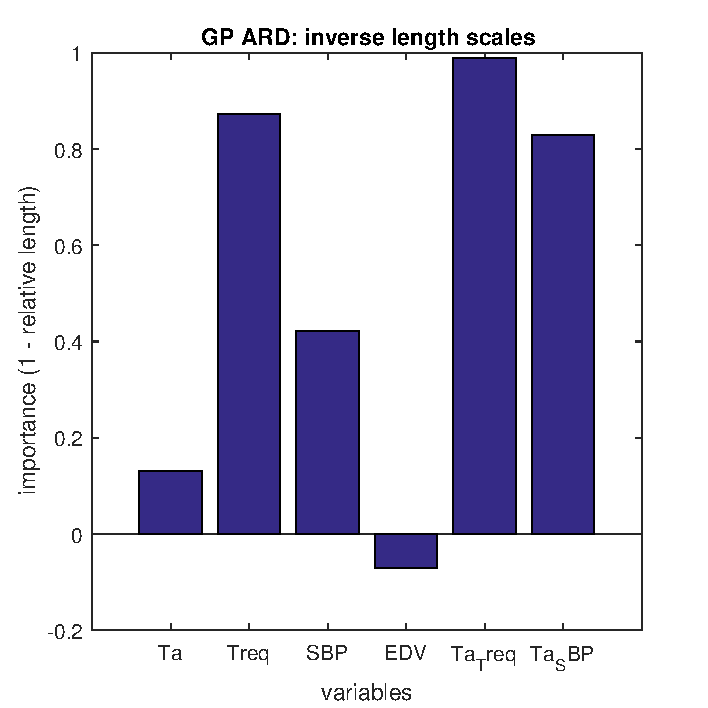
\includegraphics[width=0.3\textwidth]{Results/GP_ARD/gpard_lengthscales_dataset1.pdf}
  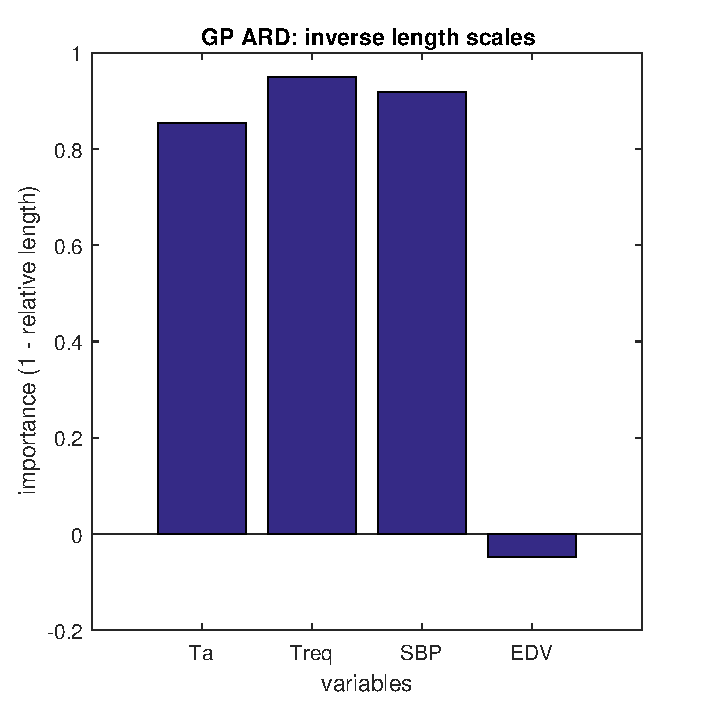
\includegraphics[width=0.3\textwidth]{Results/GP_ARD/gpard_lengthscales_dataset2.pdf}
  \includegraphics[width=0.3\textwidth]{Results/GP_ARD/gpard_lengthscales_dataset4.pdf} \\
  \includegraphics[width=0.3\textwidth]{Results/Lasso/lasso_pos_mean_coeff_datatest1.pdf}
  \includegraphics[width=0.3\textwidth]{Results/Lasso/lasso_pos_mean_coeff_datatest2.pdf}
  \includegraphics[width=0.3\textwidth]{Results/Lasso/lasso_pos_mean_coeff_datatest3.pdf} \\
  \includegraphics[width=0.3\textwidth]{Results/Random-Forest/importance_decrease_accuracy_dataset1.pdf}
  \includegraphics[width=0.3\textwidth]{Results/Random-Forest/importance_decrease_accuracy_dataset2.pdf}
  \includegraphics[width=0.3\textwidth]{Results/Random-Forest/importance_decrease_accuracy_dataset4.pdf}
  \caption{\label{fig:featureselect}\textbf{Importance of features estimated by GP-ARD and Lasso:} The top plots show the inversed relative length scales from GP-ARD and the bottom plots show the optimized regression coefficients from Lasso. Each column corresponds to one data set configuration. The GP-ARD uses a length scale parameter to determine the features with the greatest explanatory power. The length scales were inverted to make a comparison to the Lasso coefficients easier.
}
\end{figure}



\begin{figure}
   \hspace{-3mm}\includegraphics[width=0.33\textwidth]{Results/KNN/knn_sens_spec_k_dataset1.pdf}\hspace{-3mm}
  \includegraphics[width=0.33\textwidth]{Results/KNN/knn_sens_spec_k_dataset2.pdf}\hspace{-3mm}
  \includegraphics[width=0.33\textwidth]{Results/KNN/knn_sens_spec_k_dataset4.pdf}  \\
   \hspace{-3mm}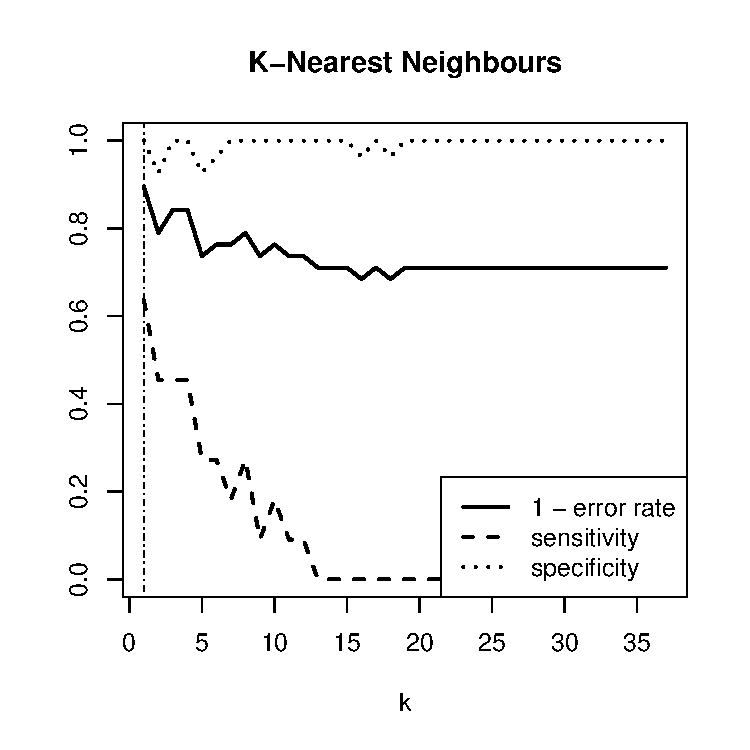
\includegraphics[width=0.33\textwidth]{Results/KNN/knn_error_k_dataset1.pdf}\hspace{-3mm}
  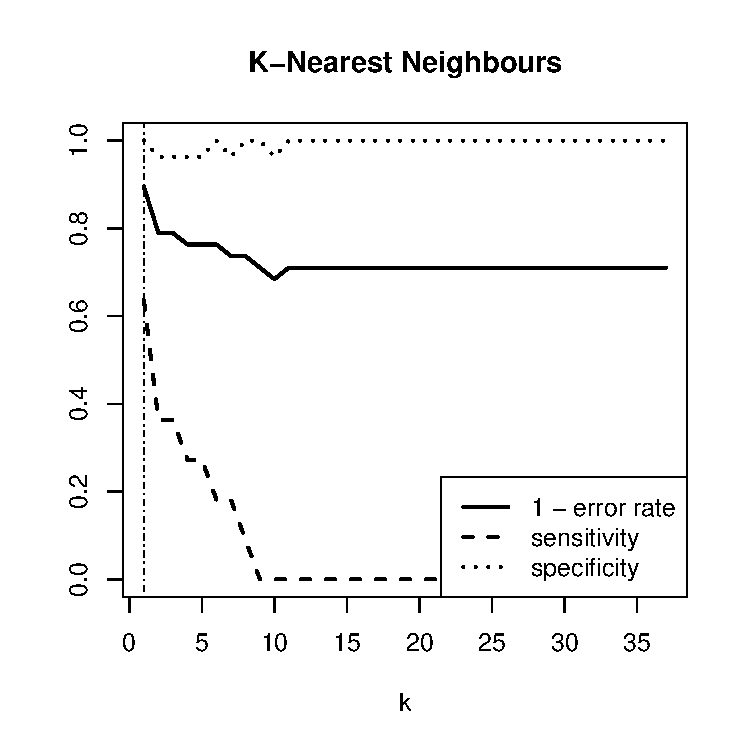
\includegraphics[width=0.33\textwidth]{Results/KNN/knn_error_k_dataset2.pdf}\hspace{-3mm}
  \includegraphics[width=0.33\textwidth]{Results/KNN/knn_error_k_dataset4.pdf}  \\
  \caption{\label{fig:knn_k}
K-nearest neighbour (KNN) with varying parameter $k = (1,\dots,n-1)$ and corresponding sensitivity (dashed line) and specificity scores (pointed line) in the top panel, and test mean squared errors (MSE) in the lower panel. The scores for each $k$ were determined with out of sample cross-validation using LOOCV (leave one out cross-validation). The left, middle and right columns correspond to the data sets $D_1$, $D_2$ and $D_3$, respectively. }
\end{figure}



\begin{figure}
  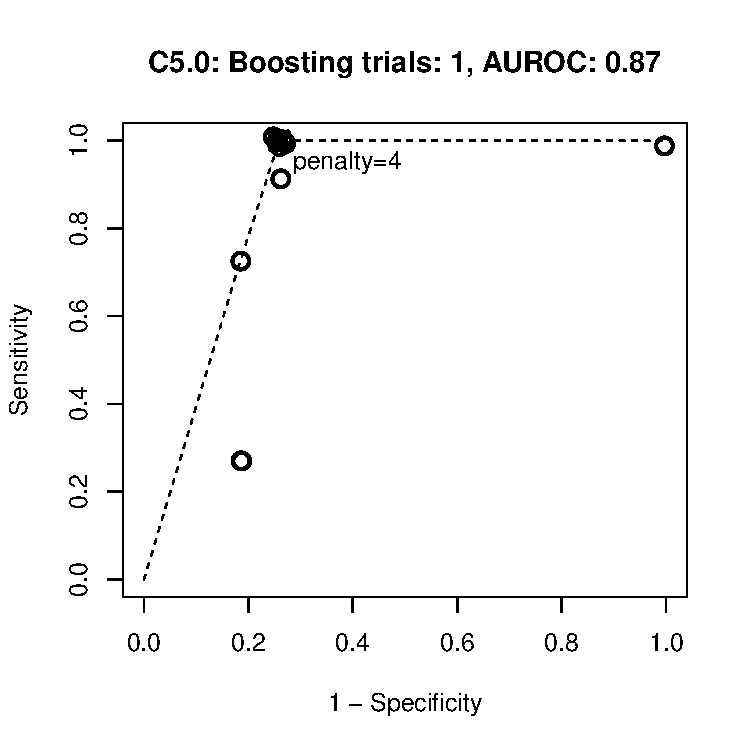
\includegraphics[width=0.33\textwidth]{Results/Decision-Tree/roc_curve_tree_boosting1_dataset1.pdf}\hspace{-0.3cm}
  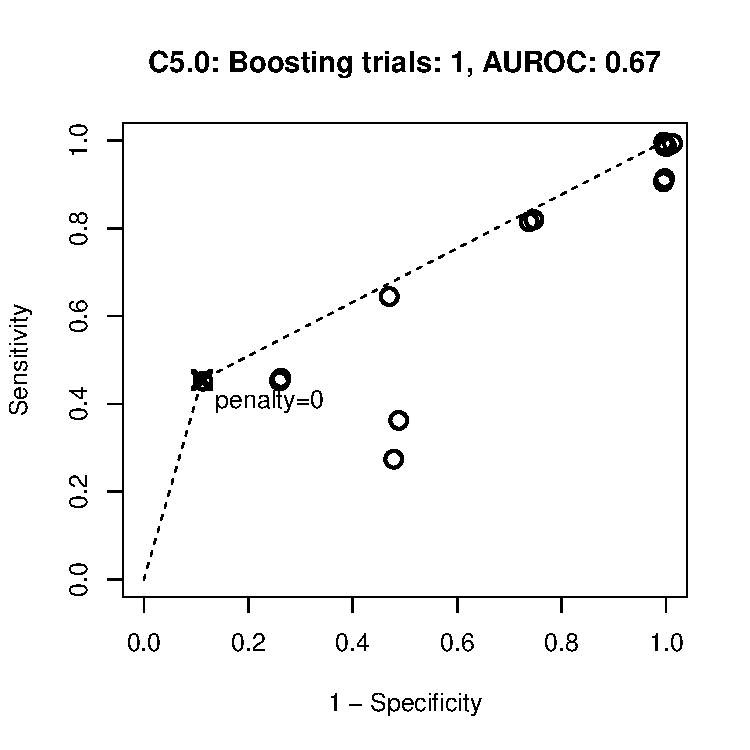
\includegraphics[width=0.33\textwidth]{Results/Decision-Tree/roc_curve_tree_boosting1_dataset2.pdf}\hspace{-0.3cm}
  \includegraphics[width=0.33\textwidth]{Results/Decision-Tree/roc_curve_tree_boosting1_dataset4.pdf} \\
  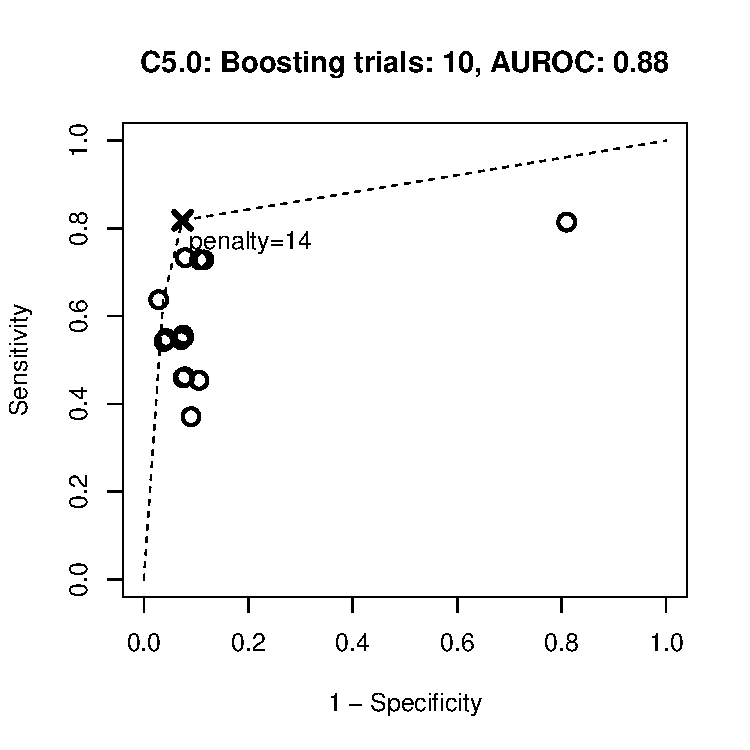
\includegraphics[width=0.33\textwidth]{Results/Decision-Tree/roc_curve_tree_boosting10_dataset1.pdf}\hspace{-0.3cm}
  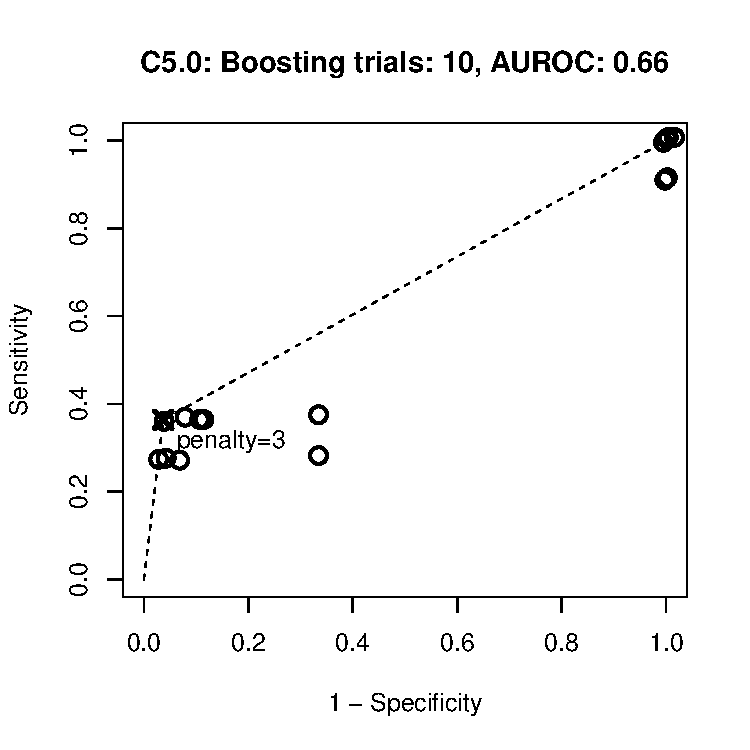
\includegraphics[width=0.33\textwidth]{Results/Decision-Tree/roc_curve_tree_boosting10_dataset2.pdf}\hspace{-0.3cm}
  \includegraphics[width=0.33\textwidth]{Results/Decision-Tree/roc_curve_tree_boosting10_dataset4.pdf} \\
  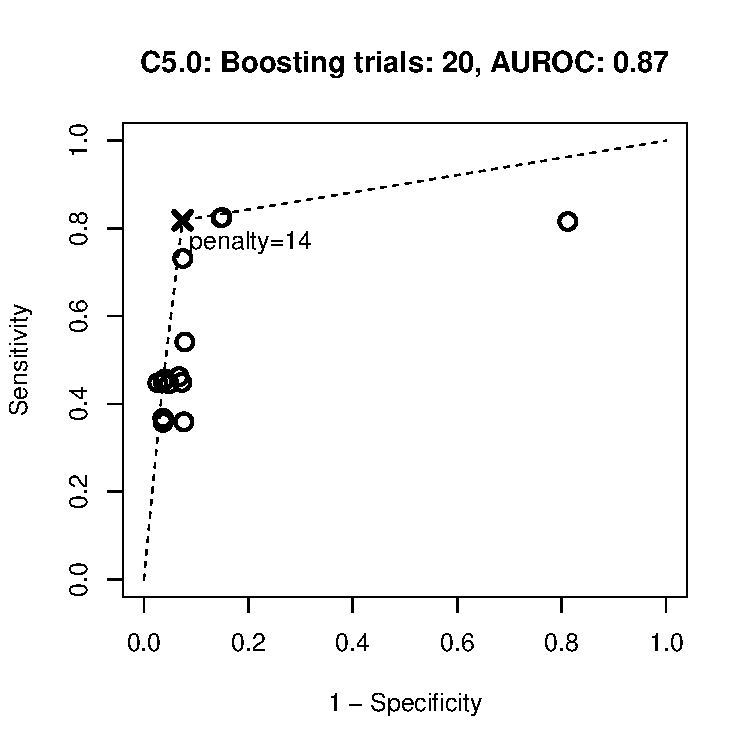
\includegraphics[width=0.33\textwidth]{Results/Decision-Tree/roc_curve_tree_boosting20_dataset1.pdf}\hspace{-0.3cm}
  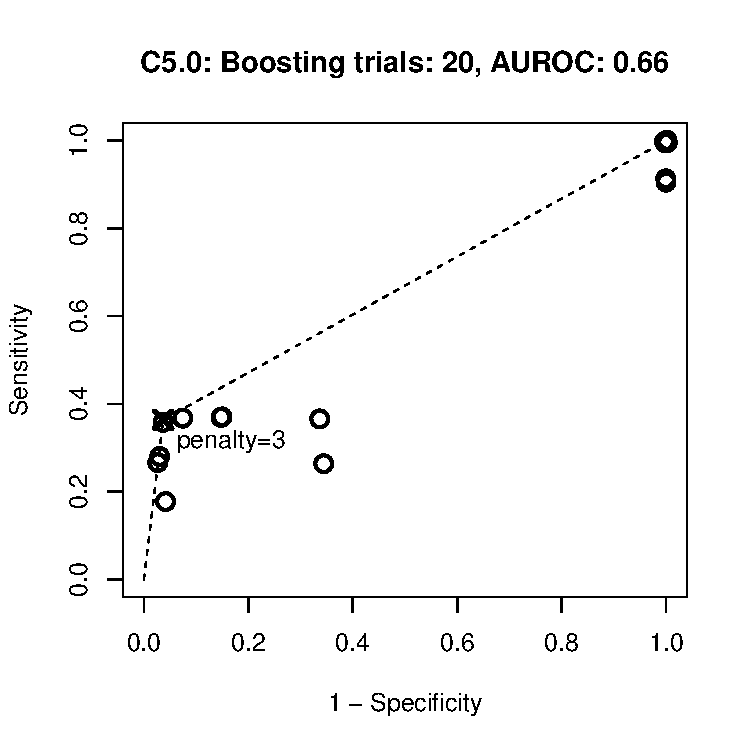
\includegraphics[width=0.33\textwidth]{Results/Decision-Tree/roc_curve_tree_boosting20_dataset2.pdf}\hspace{-0.3cm}
  \includegraphics[width=0.33\textwidth]{Results/Decision-Tree/roc_curve_tree_boosting20_dataset4.pdf} 
\caption{\label{fig:decisiontree_error_boosting}\textbf{C5.0 Decision Tree configurations:} Different settings for boosting trials and the cost penalty for three different data setups displayed in each column. The upper row shows ROC plots that lack boosting, and the lower row has a boosting of 10 trials. Each symbol in the ROC plots corresponds to cost penalty setting. The left top most point is marked with a blue triangle. LOOCV was used for each setting of boosting and error to estimate sensitivity and specificity. }
\end{figure}

\begin{figure}
  \includegraphics[width=0.33\textwidth]{Results/Decision-Tree/mse_cost_boost1_dataset1.pdf}\hspace{-0.3cm}
  \includegraphics[width=0.33\textwidth]{Results/Decision-Tree/mse_cost_boost1_dataset2.pdf}\hspace{-0.3cm}
    \includegraphics[width=0.33\textwidth]{Results/Decision-Tree/mse_cost_boost1_dataset4.pdf} \\
  \includegraphics[width=0.33\textwidth]{Results/Decision-Tree/mse_cost_boost10_dataset1.pdf}\hspace{-0.3cm}
  \includegraphics[width=0.33\textwidth]{Results/Decision-Tree/mse_cost_boost10_dataset2.pdf}\hspace{-0.3cm}
    \includegraphics[width=0.33\textwidth]{Results/Decision-Tree/mse_cost_boost10_dataset4.pdf} \\
  \includegraphics[width=0.33\textwidth]{Results/Decision-Tree/mse_cost_boost20_dataset1.pdf}\hspace{-0.3cm}
  \includegraphics[width=0.33\textwidth]{Results/Decision-Tree/mse_cost_boost20_dataset2.pdf}\hspace{-0.3cm}
    \includegraphics[width=0.33\textwidth]{Results/Decision-Tree/mse_cost_boost20_dataset4.pdf} \\
    \caption{\label{fig:decisiontree_mse}
      Mean squared error for C5.0 Decision Trees with varying error penalty. }
\end{figure}


\begin{figure}
  \includegraphics[width=0.33\textwidth]{Results/Decision-Tree/tree_boost1_error4_dataset1.pdf} \hspace{-0.3cm}
  \includegraphics[width=0.33\textwidth]{Results/Decision-Tree/tree_boost1_error0_dataset2.pdf}  \hspace{-0.3cm}
  \includegraphics[width=0.33\textwidth]{Results/Decision-Tree/tree_boost1_error4_dataset4.pdf}  \hspace{-0.3cm}
\caption{\label{fig:decisiontree}\textbf{C5.0 Decision Trees with lack of boosting:} Trees plotted for the three different data sets corresponding to the one shown in Fig.~\ref{fig:rocfinal}. }
\end{figure}


\begin{figure}
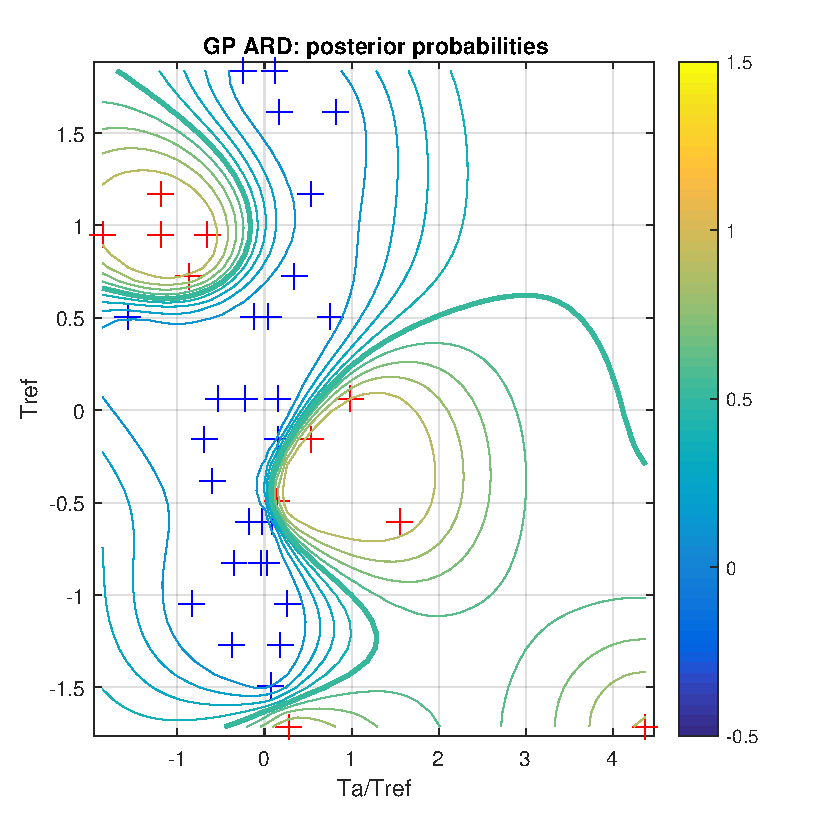
\includegraphics[width=0.48\textwidth]{Results/GP_ARD/gpard_meshprob_Ta_Tref_Tref_dataset1.pdf}
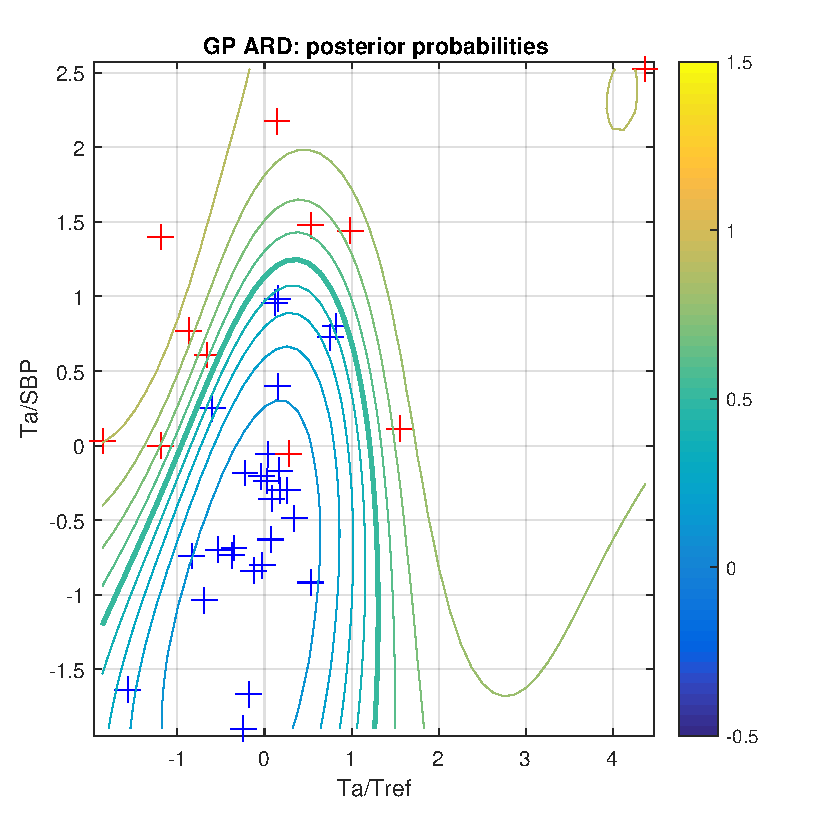
\includegraphics[width=0.48\textwidth]{Results/GP_ARD/gpard_meshprob_Ta_Tref_Ta_SBP_dataset1.pdf}
\caption{\textbf{Posterior probabilities plots of Gaussian Process - Automatic Relevance Determination (ARD):}  The two plots show the posterior probabilities mesh given the most important features estimated by GP-ARD from Fig.~\ref{fig:featureselect}, left column (data set 1): \textit{Ta/Tref}, \textit{Tref}, and \textit{SBP}.
  }
  %As lower the length scale, as more relevant the corresponding variables. The length scales are relative to the input variable range. The \textbf{right plot} shows a posterior probability mesh grid for the two most relevant variables: \textit{Ta/Tref}, \textit{Tref}, and \textit{Ta/SBP}. }
\end{figure}


%
% C5.0 Decision trees with 10 boosting trials -- looks the same as for one trial since only the first tree is plotted
%    The other 9 look obviously different (but which to pick best for decision making?)
%
%\begin{figure}
%  \includegraphics[width=0.33\textwidth]{Results/Decision-Tree/tree_boost10_error14_dataset1.pdf}
%  \includegraphics[width=0.33\textwidth]{Results/Decision-Tree/tree_boost10_error2_dataset2.pdf}
%  \includegraphics[width=0.33\textwidth]{Results/Decision-Tree/tree_boost10_error14_dataset4.pdf}
%\caption{\textbf{C5.0 Decision Trees with 10 boosting trials:} Trees plotted for the three different data setups corresponding to the one shown in Fig.~\ref{fig:rocfinal}. \textit{Note that two of the trees are simplier than the one we have seen before (Rosalind). The difference is the new data and a lack of boosting.}}
%\end{figure}

\begin{figure}
\includegraphics[width=0.33\textwidth]{Results/roc_curve_datatest1.pdf} \hspace{-0.3cm} 
\includegraphics[width=0.33\textwidth]{Results/roc_curve_datatest2.pdf} \hspace{-0.3cm}
\includegraphics[width=0.33\textwidth]{Results/roc_curve_datatest3.pdf}
\caption{
  \label{fig:rocfinal}\textbf{Overall classification performance given three different data setups:} The area under the ROC curve (AUROC) is calculated from the area under the convex hull that connects the best performing methods. The specificity and sensitivity score for each method was estimated with LOOCV. The left plot uses the features from data set $D_1$, the middle plot shows the performance for data set $D_2$, and the right plot for data set $D_3$.}
\end{figure}





\end{document}
